\begin{frame}{Vetores de bits - access}
    Sequência de $n$ elementos sobre o alfabeto $\Sigma = \{0,1\}$, no qual podem ser realizadas as seguintes operações \citep{book-compact-data-structures}:
        \vspace{0.5cm}
        \begin{itemize}
            \item $access(BV,i)$: retorna o i-ésimo bit do vetor BV, com $0 \leq i < n$;
            \vspace{0.5cm}
            
            Exemplo: $access(BV,10)$
            
            \begin{figure}[h!]
                \centering
                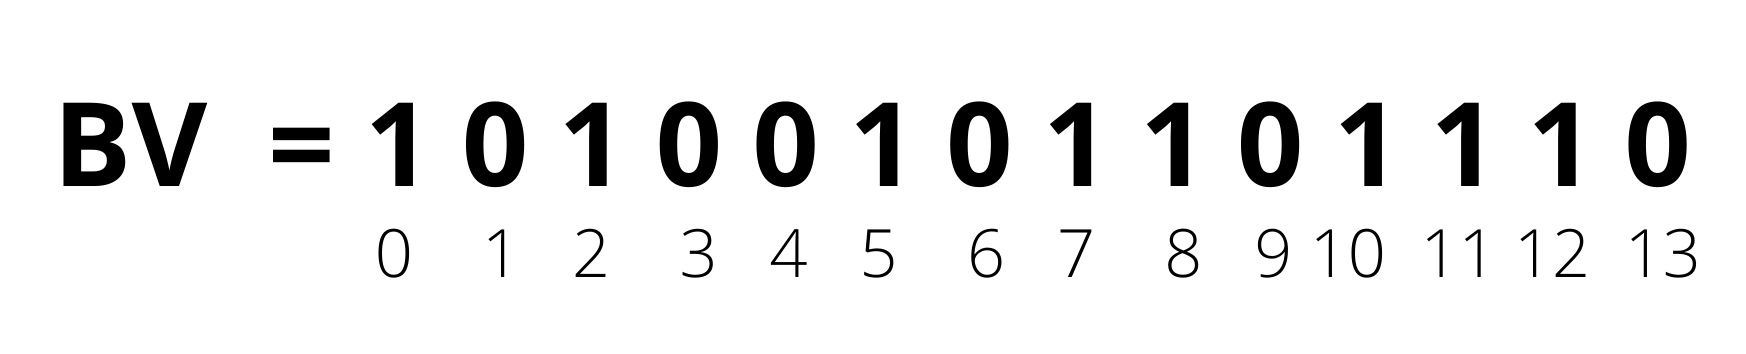
\includegraphics[scale=0.5]{images/bitvector.png}
            \end{figure} 
        \end{itemize}
    \end{frame}
    
    \begin{frame}{Vetores de bits - access}
        Exemplo: $access(BV,10)=1$
        \begin{figure}[h!]
            \centering
            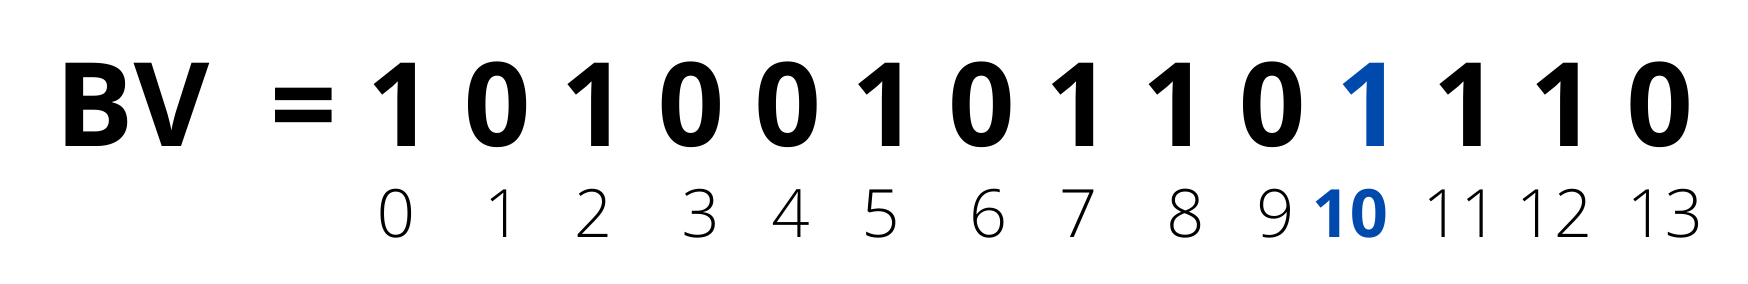
\includegraphics[scale=0.7]{images/access-res.png}
        \end{figure} 
    \end{frame}
    
    
    \begin{frame}{Vetores de bits - rank}
    Sequência de $n$ elementos sobre o alfabeto $\Sigma = \{0,1\}$, no qual podem ser realizadas as seguintes operações \citep{book-compact-data-structures}:
        \vspace{0.5cm}
        \begin{itemize} 
            \item $rank_v(BV,i)$: seja $v \in \{0,1\}$, e $0 \leq i < n$, retorna o número de ocorrências de $v$ no intervalo $BV[0,i]$.
            \vspace{0.5cm}
            
            Exemplo: $rank_0(BV,8)$
            
            \begin{figure}[h!]
                \centering
                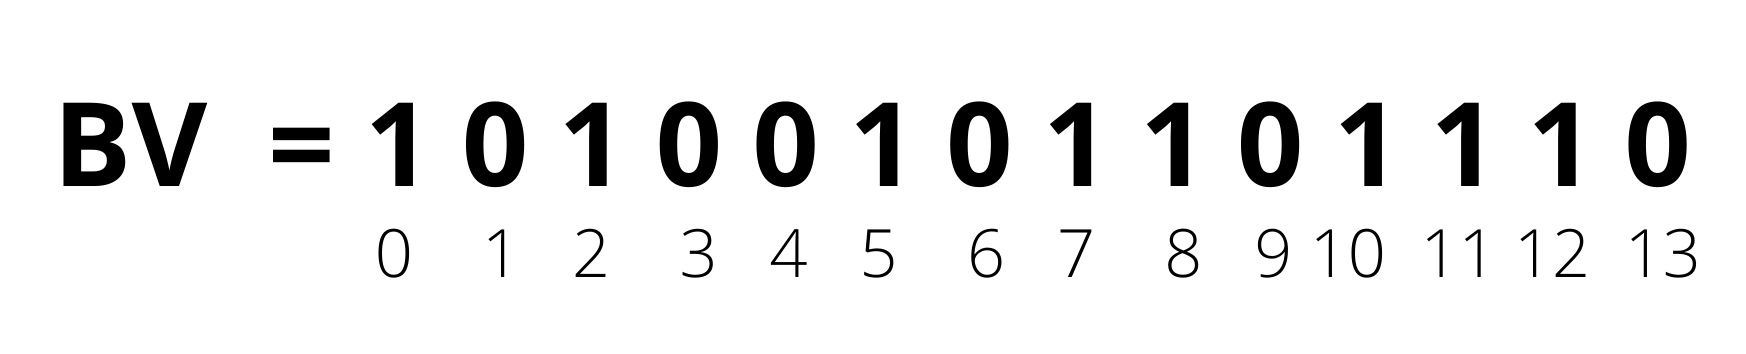
\includegraphics[scale=0.5]{images/bitvector.png}
            \end{figure} 
        \end{itemize}
    \end{frame}
    
    \begin{frame}{Vetores de bits - rank}
        Exemplo: $rank_0(BV,8)=4$
        \begin{figure}[h!]
            \centering
            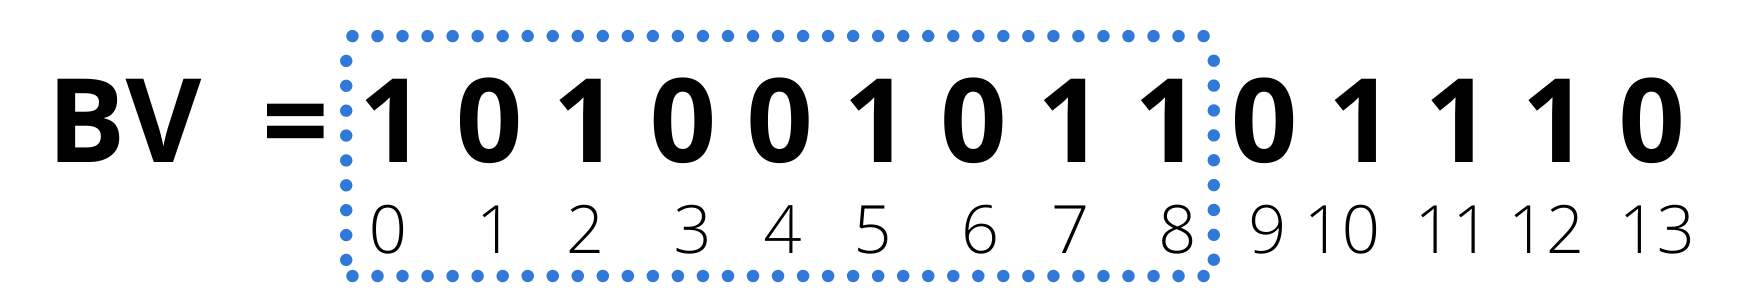
\includegraphics[scale=0.7]{images/rank-res.png}
        \end{figure} 
    \end{frame}
    
    \begin{frame}{Vetores de bits - select}
    Sequência de $n$ elementos sobre o alfabeto $\Sigma = \{0,1\}$, no qual podem ser realizadas as seguintes operações \citep{book-compact-data-structures}:
        \vspace{0.5cm}
        \begin{itemize} 
              \item $select_v(BV,i)$: dado $v \in \{0,1\}$ e $i \geq 1$, retorna a posição do i-ésimo bit $v$ em $BV[0,n-1]$.
              \vspace{0.5cm}
            
                Exemplo: $select_1(BV,8)$
            
                \begin{figure}[h!]
                    \centering
                    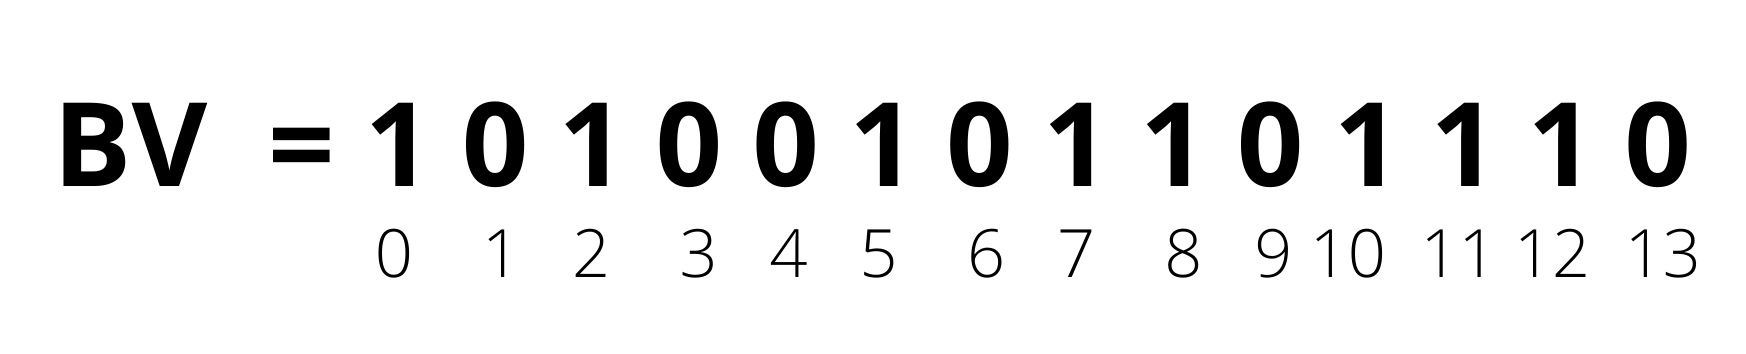
\includegraphics[scale=0.5]{images/bitvector.png}
                \end{figure} 
        \end{itemize}
    \end{frame}
    
    \begin{frame}{Vetores de bits - select}
        Exemplo: $select_1(BV,8)=12$
        \begin{figure}[h!]
            \centering
            
\includegraphics[scale=0.7]{images/select-res.png}
        \end{figure} 
    \end{frame}